\documentclass[../MA_Thesis.tex]{subfiles}
\renewcommand{\baselinestretch}{1.5} 
\usepackage{hyperref}
\usepackage{csquotes}
\usepackage{float}
\usepackage{threeparttable}  % for table notes
\usepackage{booktabs}        % for \toprule, \midrule, \bottomrule

\begin{document}
\subsection*{Manipulation Check: Mood Induction}
To verify that the mood induction procedure successfully manipulated participants’ mood states along both the arousal and valence dimensions, I conducted one-way ANOVAs with mood group (\textit{High-Arousal Positive Mood}, \textit{Low-Arousal Positive Mood}, and
\textit{Neutral Control}) as the between-subjects factor.

For arousal ratings, a one-way ANOVA revealed a significant effect of induced mood condition, $F(2, 87) = 6.86$, $p = .0017$, with a moderate effect size ($\eta^2 = .14$). Furthermore, post-hoc Tukey tests showed that participants in the \textit{High-Arousal Positive Mood} group (M = 6.70, SD = 1.02) reported significantly higher arousal than those in the \textit{Neutral Control} group (M = 4.05, SD = 1.12; $p = .0021$) and the \textit{Low-Arousal Positive Mood} group (M = 4.53, SD = 1.09; $p = .0171$). No significant difference was observed between the \textit{Neutral Control} and \textit{Low-Arousal Positive Mood} groups ($p = .7641$; see Figure). 

For valence ratings, a one-way ANOVA also showed a significant group difference, $F(2, 87) = 4.44$, $p = .0146$, with a moderate effect size ($\eta^2 = .09$). Moreover, post-hoc Tukey tests revealed that the \textit{High-Arousal Positive Mood} group (M = 2.91, SD = 0.96) reported significantly higher valence than the \textit{Neutral Control} group (M = 1.24, SD = 1.24; $p = .0167$), whereas the \textit{Low-Arousal Positive Mood} group (M = 2.16, SD = 1.10) did not significantly differ from either group ($ps > .05$; see Figure). 

Overall, the experimental mood induction procedure using three validated film clips achieved the anticipated mood manipulation results. For the two positive valence groups, there was a significant difference in arousal ratings, whereas the valence ratings did not significantly differ. This pattern supports the intended orthogonal manipulation of arousal while holding valence constant, allowing for a more focused investigation of arousal's unique effects on subsequent creative processes. Meanwhile, the significant differences in both arousal and valence ratings between the \textit{High-Arousal Positive Mood} and \textit{Neutral Control} groups confirm the successful induction of a distinctly activated positive affective state in the high-arousal condition.

% \begin{figure}[H]
%   \centering
%   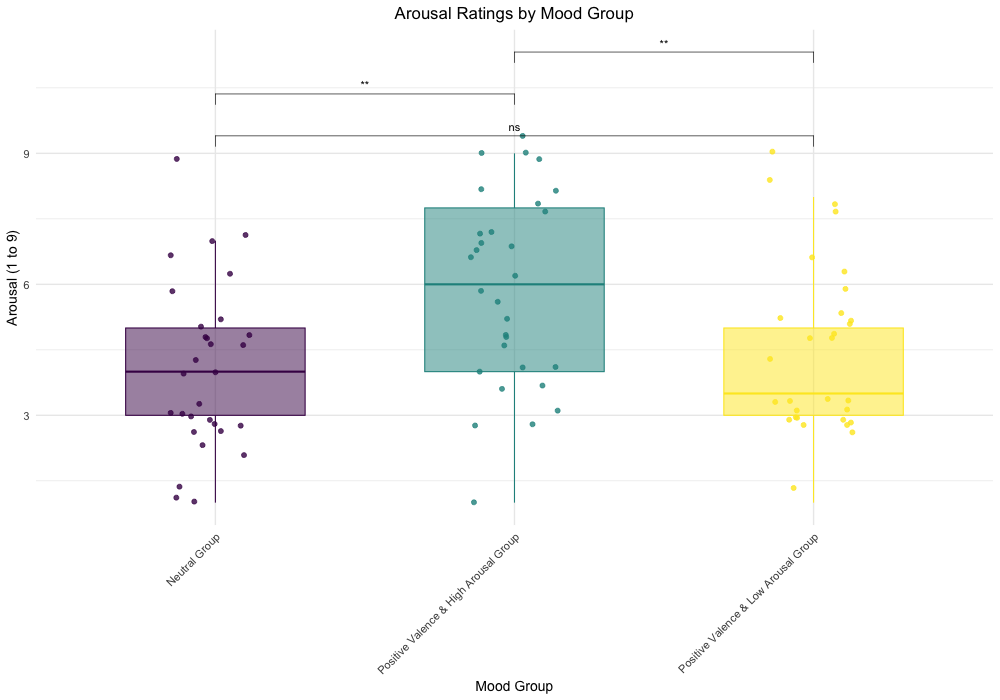
\includegraphics[width=0.75\textwidth]{../analysis/results/mood_induction_check/arousal_by_group.png}
%   \caption{Boxplot of arousal ratings by mood condition}
%   \label{fig:arousal_group}
% \end{figure}

% \begin{figure}[H]
%   \centering
%   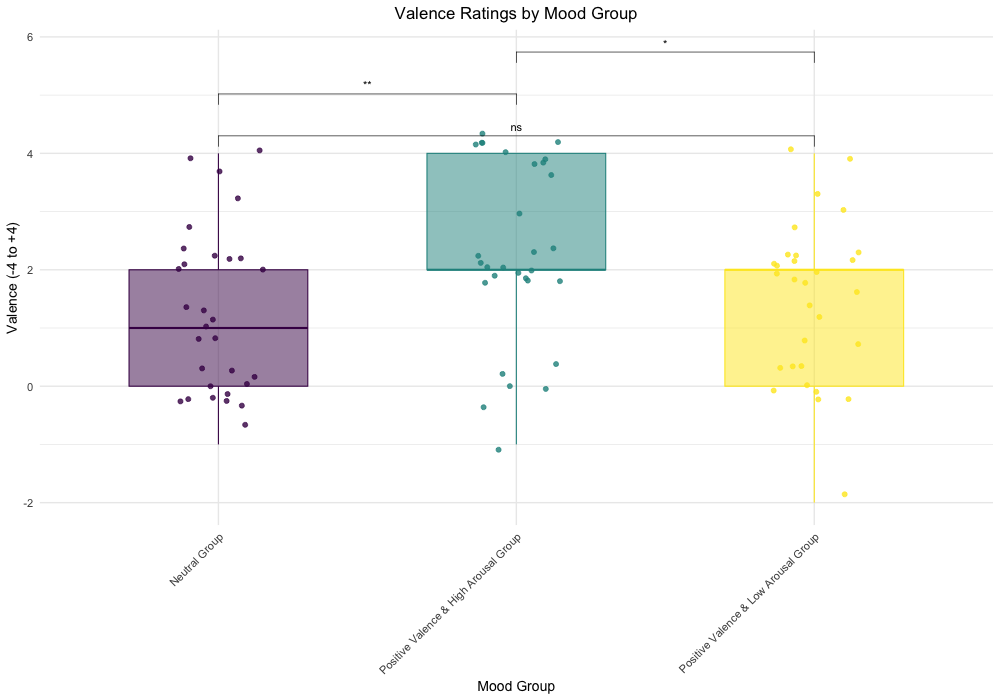
\includegraphics[width=0.75\textwidth]{results/mood_induction_check/valence_by_group.png}
%   \caption{Boxplot of valence ratings by mood condition}
%   \label{fig:valence_group}
% \end{figure}

\subsection*{Descriptive Statistics}

Means and standard deviations for all flexibility measures and the originality measure are presented in Table~\ref{tab:descriptive_stats}. Overall, the flexibility metrics showed subtle variation across mood conditions. 

\begin{table}[H]
\centering
\begin{threeparttable}
\caption{Descriptive Statistics by Mood Condition (Mean (SD))}
\label{tab:descriptive_stats}
\begin{tabular}{lccc}
\toprule
\textbf{Measure} & \textbf{Neutral Group} & \textbf{High Arousal Group} & \textbf{Low Arousal Group} \\
\midrule
Avg. Entropy & 1.77 (0.09) & 1.78 (0.07) & 1.74 (0.10) \\
Avg. Bhatt. Dist. & 2.51 (0.29) & 2.50 (0.25) & 2.45 (0.28) \\
Inflect. Prop. Entropy & 0.41 (0.18) & 0.42 (0.17) & 0.45 (0.17) \\
Inflect. Prop. Bhatt & 0.42 (0.18) & 0.43 (0.16) & 0.44 (0.20) \\
DSI & 0.59 (0.28) & 0.66 (0.22) & 0.58 (0.30) \\
AuDrA & 0.37 (0.10) & 0.36 (0.10) & 0.37 (0.11) \\
\bottomrule
\end{tabular}
\begin{tablenotes}[flushleft]
\small
\item \textit{Note.} Avg. Entropy = Average Entropy; Avg. Bhatt. Dist. = Average Bhattacharyya Distance; Inflect. Prop. Entropy = Inflection Proportion of Entropy; Inflect. Prop. Bhatt = Inflection Proportion of Bhattacharyya Distance; DSI = Divergent Semantic Integration; AuDrA = Automated Drawing Assessment (Originality Score).
\end{tablenotes}
\end{threeparttable}
\end{table}

Average entropy was comparable across groups, with the \textit{High Arousal} group showing the highest entropy (M = 1.78, SD = 0.07), followed closely by the \textit{Neutral} group (M = 1.77, SD = 0.09) and the \textit{Low Arousal} group (M = 1.74, SD = 0.10). A similar pattern was observed for average Bhattacharyya distance. 

In contrast, \textit{DSI} was highest in the \textit{High Arousal} group (M = 0.66, SD = 0.22), slightly higher than the \textit{Neutral} (M = 0.59, SD = 0.28) and \textit{Low Arousal} (M = 0.58, SD = 0.30) groups. Interestingly, inflection proportions (both entropy and Bhattacharyya-based) were slightly elevated in the \textit{Low Arousal} group, suggesting greater within-trial flexibility switching.

Originality scores, as measured by AuDrA, were remarkably consistent across groups (M = 0.36–0.37, SD ≈ 0.10), with no meaningful variation.

\end{document}